\section{Dental caries}

\subsection{Epidemiology}

Diseases of the oral cavity are amongst the most prevalent conditions worldwide and they are known to be associated with a substantial health and economic burden \citep{peres2019, gbd2017}. In fact, dental caries (often referred to as "tooth decay" or "cavities") is the most common chronic disease affecting children in the United States (US), with recent estimates indicating that over a quarter of children aged between 2 to 11 years have experienced the disease \citep{oral2000, bashir2022}. The epidemiology of dental caries is well-characterised and it is known that the condition is distributed in a highly inequitable manner, with individuals from minority ethnic groups, poorer households, and lower educational attainment carrying a disproportionate burden of disease \citep{bashir2021, bashir2022}.

Dental caries has a number of deleterious effects on the day-to-day functioning of children, including impairments to physical, mental, and social functioning, problems with eating and sleeping, and a significant increase in the risk of experiencing pain  \citep{cunnion2010, singh2020, boeira2012}. It has been shown that children with poor oral health are more likely to miss school due to dental pain, and these absences are associated with poorer academic performance, highlighting the multifaceted manner in which oral pathology takes a toll on children \citep{jackson2011}. Given the high prevalence of disease, it comes as no surprise that the economic burden of dental caries is vast. It is estimated that over \$220 million in productivity losses in the US are attributable to dental caries in the primary dentition (i.e., "baby teeth"), and over \$5.3 billion are attributable to dental caries in the permanent dentition (i.e., "adult teeth") \citep{righolt2018}.

\subsection{Aetiology}

In order to understand how dental caries develops, it is important to appreciate the basics of tooth anatomy. The portion of the tooth which lies above the gum is known as the crown, whilst the portion which lies below is known as the root, as shown in \autoref{fig:anatomy}. The crown of the tooth comprises three types of tissue: (i) the outermost surface is made up of enamel, which is the hardest and most mineralised tissue across all vertebrate species, with 95\% of enamel being composed of mineralised hydroxyapatite crystals, (ii) beneath the enamel lies the dentine, which is a more porous structure that is made up of 70\% mineralised tissue, (iii) in the centre lies the pulp, which is the neurovascular tissue providing sensation to the tooth \citep{lacruz2017, goldberg2011}.

\begin{figure}[ht]
\centering
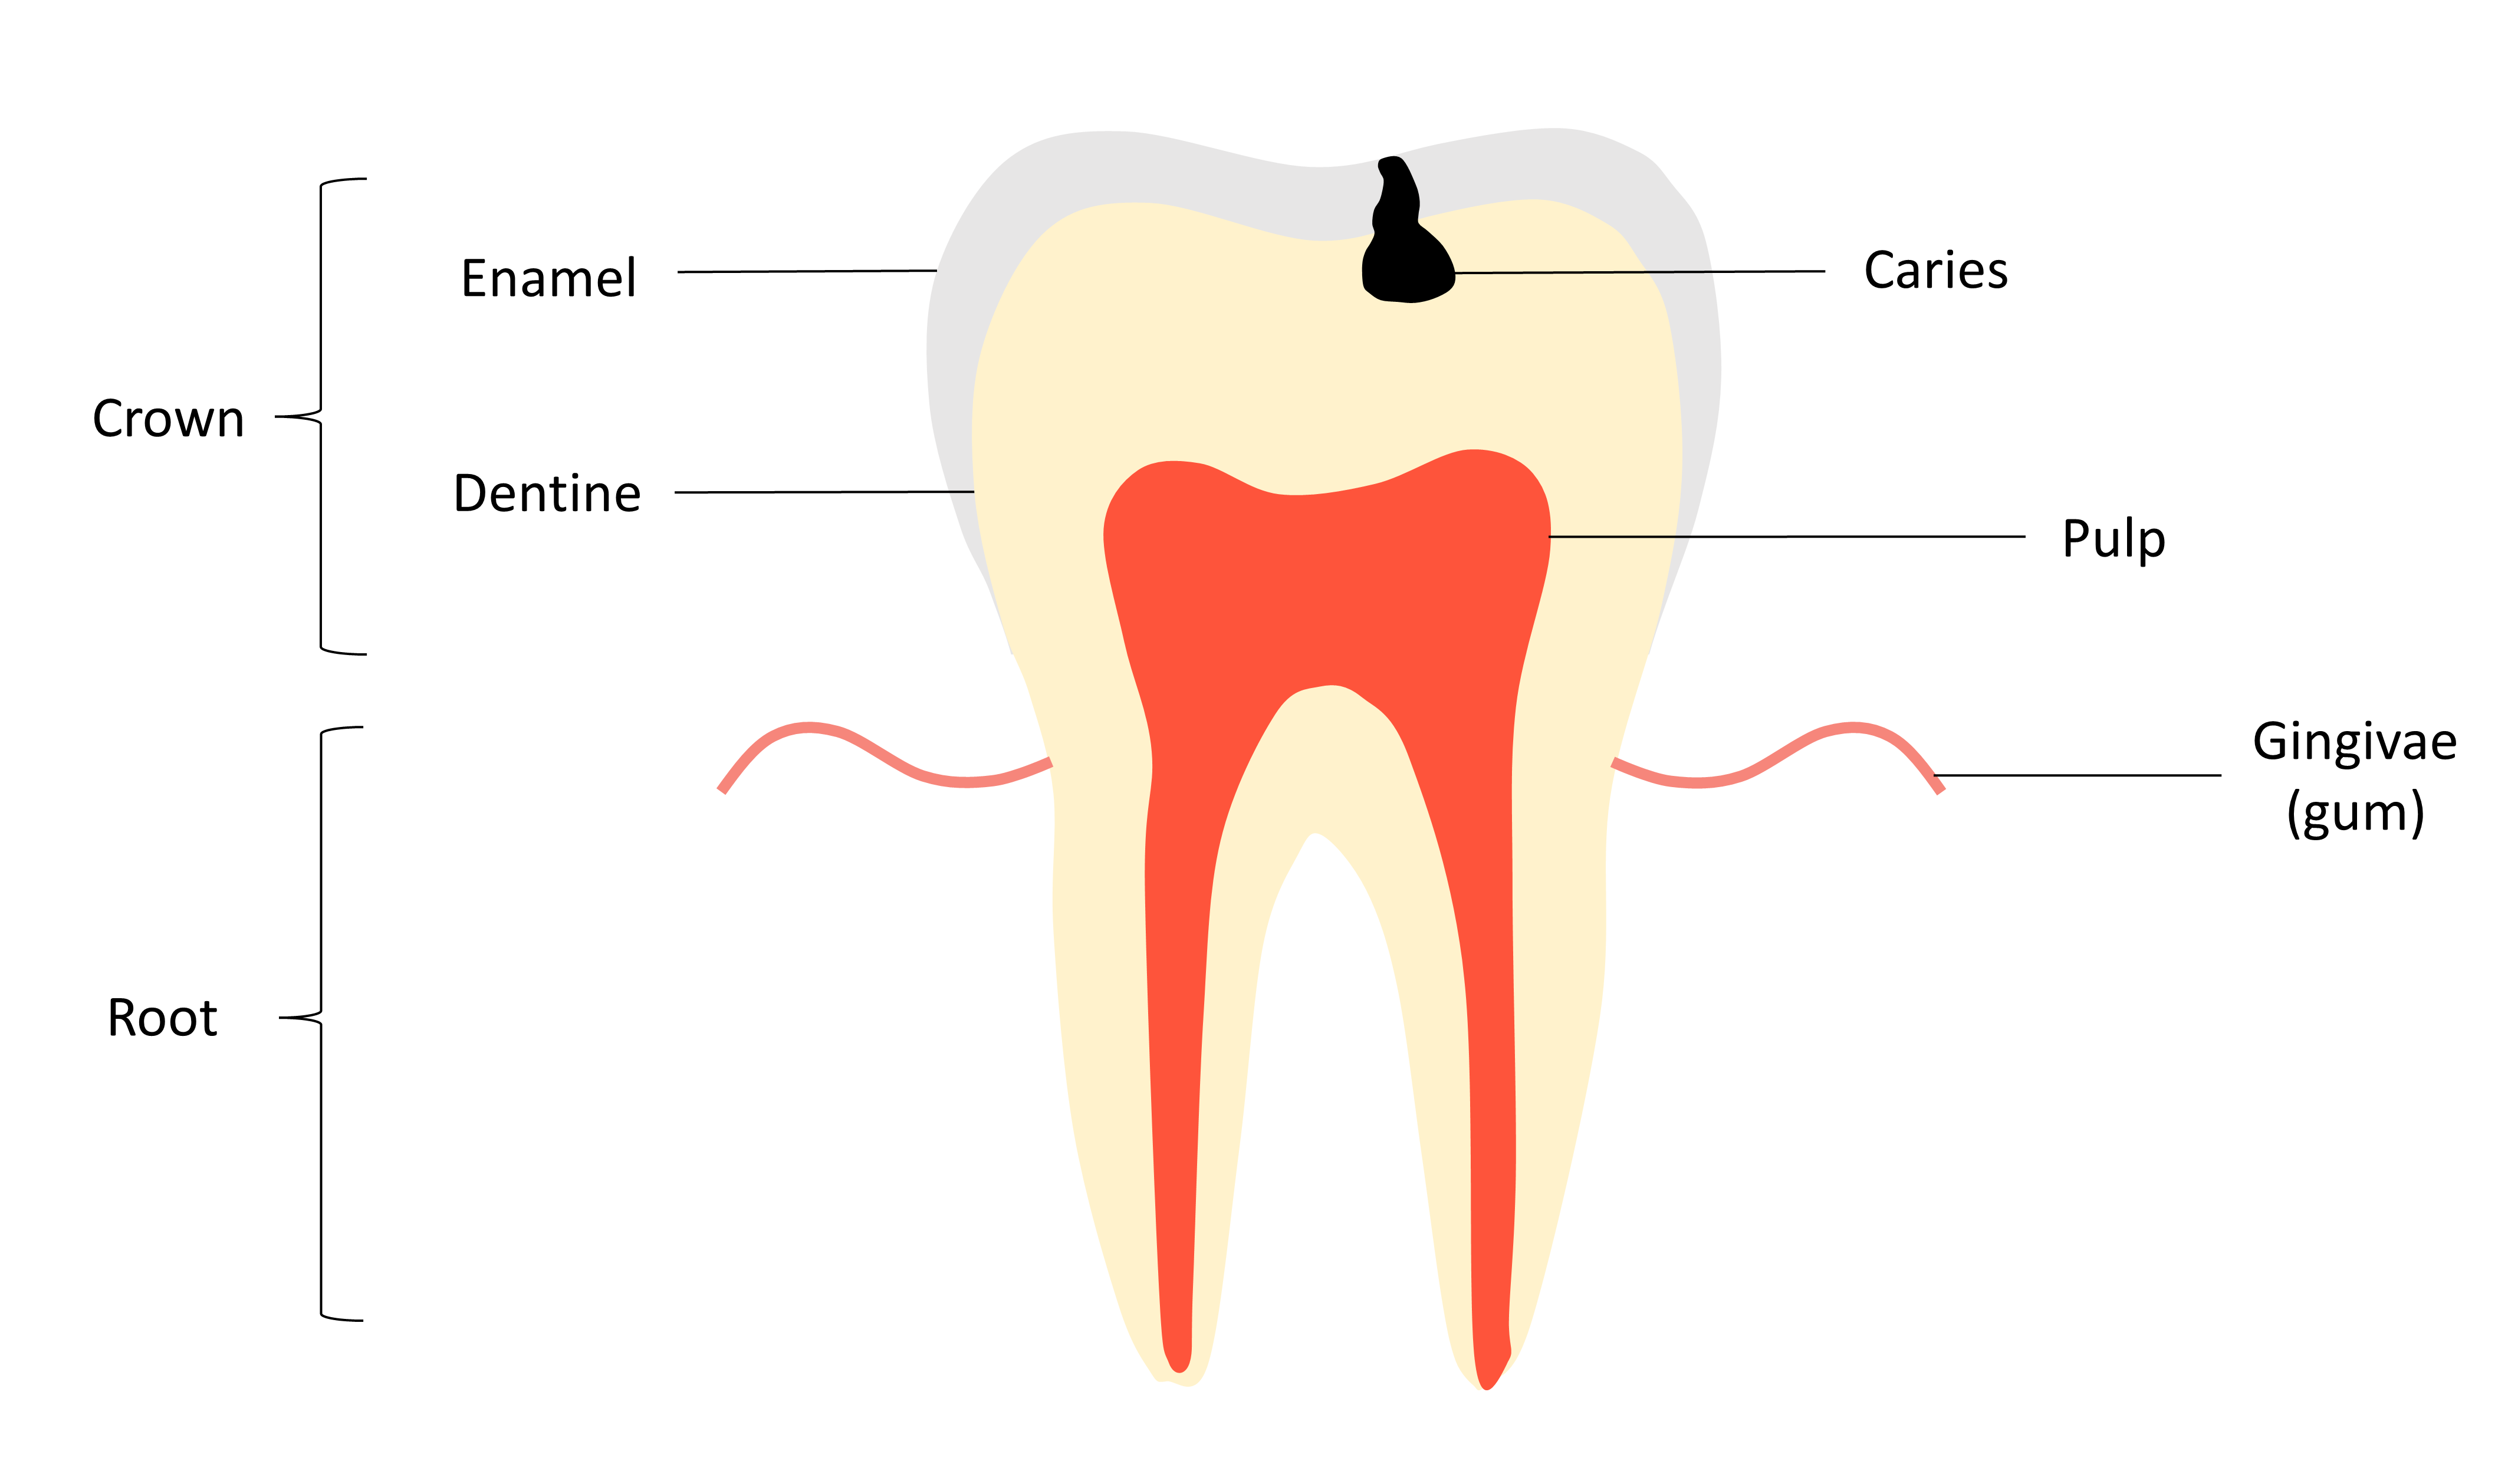
\includegraphics[scale = 0.25]{images/tooth}
\caption{Tooth anatomy and a developing carious lesion.}
\label{fig:anatomy}
\end{figure}

There are three key components which are implicated in the aetiology of dental caries:

\begin{enumerate}
\item Sugar intake
\item Oral hygiene
\item Fluoride exposure
\end{enumerate}

It is true that these are not the only factors involved e.g., there are developmental conditions affecting formation of enamel and dentine, thus predisposing individuals to dental caries \citep{costa2017}. However, such conditions are relatively rare, and in the vast majority of cases it is a combination of excess sugar intake and inadequate oral hygiene practices which give rise to the disease process \citep{crawford2007, barron2008, pitts2017}. Fluoride exposure also plays a critical role in the pathophysiology of dental caries, and this will be discussed in tandem with oral hygiene, as the two are interconnected.

Dental caries will not occur in the absence of frequent exposure to dietary carbohydrates (namely, free sugars). Pathogenic bacteria inhabit the tooth surface and digest these sugars to produce acidic metabolites which demineralise the enamel, facilitating entry of the microorganisms into the underlying dentine \citep{pitts2017}. Once this stage is reached, the pathogens can spread rapidly through the dentine due to its porous nature \citep{pitts2017}. If the disease process breaches the pulpal tissue, individuals will typically experience significant pain and require extensive treatment of the tooth in order to avoid a dental extraction \citep{iqbal2007}.

Maintaining a good oral hygiene routine is key for two reasons: (i) toothbrushing allows for manual disruption of the pathogenic microbiota on the tooth surface, (ii) toothbrushing allows for deposition of fluoridated toothpaste onto the tooth surface \citep{pitts2017}. It is difficult to overemphasise just how crucial fluoride is in modifying the disease process. Fluoride ions integrate into the hydroxyapatite crystals which make up the tooth structure, giving rise to hydroxyfluorapatite, which has an increased resistance to acidic demineralisation and promotes remineralisation \citep{buzalaf2011}. Not only this, but fluoride inhibits the ability of the pathogenic agents to metabolise sugars and adhere to the tooth surface \citep{buzalaf2011, liao2017}. The most common routes of fluoride exposure are typically from toothpaste, within drinking water, and from high-concentration varnishes applied by dentists.

\subsection{Treatment}

One key factor which distinguishes dental caries from many other chronic childhood diseases is the fact that it is almost entirely preventable. Not only is it preventable, but there are a range of treatment options which are known to be highly efficacious in halting, and sometimes reversing, progression of the disease.

Contemporary disease management centres heavily around prevention. The risk factors which predispose individuals to dental caries are modifiable, so educating patients on the aetiology of dental caries is key in preventing disease occurrence. Systematic reviews have shown that restricting sugar intake is associated with a reduction in disease prevalence, incidence, and severity \citep{moynihan2017}. In addition, the application of topical fluoride (in virtually all forms) has been shown to be highly efficacious as a preventive measure, and this is an intervention which is easily administered by dentists \citep{weyant2013}. Interestingly, improvements in oral hygiene in the absence of fluoride do not appear to have any substantial benefit in reducing caries risk \citep{hujoel2018}. This combination of reduced sugar intake and increased fluoride exposure forms the cornerstone of disease prevention. 

Once disease is established, then active intervention is indicated. Historically, a "drill-and-fill" approach was common, where treatment focused on drilling into diseased lesions to remove the infected tooth structure, followed by placement of a restoration. This is not the case in modern-day practice, where a minimally invasive approach is now preferred \citep{walsh2013}. Topical agents, such as high-fluoride varnishes and sealants, can be used to arrest incipient lesions and induce remineralisation of the enamel \citep{walsh2013}. Of course, this is not applicable to all cases. When disease has spread deep into the dentine, then it is necessary to drill into the lesion and subsequently restore the tooth. Furthermore, when the pulp tissue becomes involved, more extensive endodontic treatment (i.e., root canal treatment) is typically required.

Overall, modern treatment principles for dental caries are dictated by the extent of disease and the specific risk factors which a patient presents with. If the disease is left untreated for long enough, then minimally invasive treatment is no longer an option and more invasive procedures are required. If this is the case, it is not uncommon for patients to have experienced substantial pain and discomfort by this point \citep{iqbal2007}.

In a clinical setting, practitioners will carry out detailed history-taking to understand patients' oral hygiene routines and diet habits, alongside rigorous clinical examination, to identify individuals where targeted preventive measures should be taken. On the other hand, epidemiologists have extensively evaluated the social determinants of disease, such as education and income, and there is now insurmountable evidence highlighting the disparate nature in which the disease afflicts individuals of lower socioeconomic status \citep{baker2014}. However, on the background of a shifting political landscape, underexplored risk factors have recently been bought to light, with immigration being at the forefront of investigation for many health researchers \citep{abubakr2018}.

\section{Immigration and health}

\subsection{Introduction}

Migrants can be defined as individuals who have moved away from their habitual place of residence; as of 2018, approximately one-seventh of the world population met this definition \citep{abubakr2018}. Human migration has been a key component in the evolution of culture, economies, and mankind as a species. It is only in recent times that the lens has been shifted onto migration as a fundamental determinant of health. International law dictates that all migrants have the right to the "highest attainable standard of health", yet the evidence demonstrates that this is often not the case \citep{un1976, abubakr2018}. Migrants are also entitled to the fundamental socioeconomic and political rights which determine health outcomes, such as clean water and non-discriminatory treatment \citep{abubakr2018}. Yet, many governments implement policies which infringe on these rights. In some cases, we even see persecution of individuals seeking asylum, with the 2018 US government's policies that resulted in separation of children from their parents being an obvious example of this occurring in the developed world \citep{abubakr2018}. The global distribution of migrants is illustrated in \autoref{fig:map}.

\afterpage{\clearpage}

\begin{sidewaysfigure}[ht]
\includegraphics[scale = 0.15]{images/migration_map}
\caption{Distribution of migrants as of 2015, where it can be seen that people tend to migrate to higher-income countries. Taken from the \emph{Lancet} Migration Collaboration at: \url{https://www.migrationandhealth.org/data}.}
\label{fig:map}
\end{sidewaysfigure}

\subsection{Challenges}

The full host of reasons as to why migration affects health outcomes is too complex and multifaceted to address comprehensively, but we will present a brief overview here. Essentially, there are four factors which govern migrant health: (i) politics, (ii) culture, (iii) environment, and (iv) structural disparities \citep{abubakr2018}. 

\subsubsection{Politics}

Migration is a political hotbed, with migrant-blaming becoming a staple in the repertoire of many politicians. A commission by the \emph{Lancet} found that this has led to a clash between the health sector's goal of non-prejudicial and equally accessible healthcare for all, versus the aims of state and corporate entities who are driven by political motivations \citep{ottersen2014}. 

\subsubsection{Culture}

Culture is an extremely broad term referring to a combination of knowledge, beliefs, and behaviours that characterise people or societies \citep{heyes2020}. An individual's culture is a dynamic state which will inevitably be influenced by migration \citep{abubakr2018}. The very process of undergoing migration, as well as the new locations, may alter how individuals care for themselves and those around them, as well as their views on healthcare, and the manner in which they choose to engage with healthcare systems surrounding them \citep{abubakr2018}. 

\subsubsection{Environment}

Environments that migrants move to (and from) will have different rates of events which produce adverse health outcomes, such as infectious diseases, conflicts, droughts, famine, and natural disasters \citep{abubakr2018}. These same factors may also act as drivers of migration, temporarily or permanently forcing individuals out of their habitual place of residence.

\subsubsection{Structural disparities}

Structural disparities are numerous, and these essentially refer to systematic differences between the physical and social conditions endured by migrants and non-migrants. Migrant children may face a disruption of education and subsequent difficulty in accessing schools, there may be disparities in working conditions whereby migrants undertake labour which is unsafe and a hazard to health, and there may be disparities in access to healthcare whereby migrants live in locations which are physically disadvantageous for accessing the local healthcare resources \citep{abubakr2018}.

\subsection{Oral health}

There is a growing body of evidence suggesting that oral health is one of the many aspects of health which is affected by migration. A recent systematic review found that migrants in Europe have a higher prevalence of dental caries and periodontal disease (i.e., gum disease), compared to their native-born counterparts, whilst other studies indicate that migrants have a poorer oral health-related quality of life \citep{lauritano2021, aarabi2022}. Some of the key factors which have been found to mediate this relationship include: cost, cultural misunderstandings, language, poorer oral health-related education and practices, and reduced access to oral healthcare services amongst non-native born individuals \citep{pabbla2021, riggs2014, newton2001}. 

Of the evidence available, only a small proportion pertains to the US population. This is surprising considering the fact that there are over 50 million non-native born individuals in the country \citep{un2019}. This is over 4 times more than Germany (the country with the second largest number of migrants); in fact, the entirety of Western Europe is home to around 30 million migrants, which is still 20 million less than the US \citep{un2019}. Therefore, understanding oral health amongst migrants living in the US is of great interest.

\section{Objectives}

The aims of this dissertation are: (i) to investigate how migration (i.e., nativity status) is associated with dental caries amongst children in the US population, (ii) to understand how statistical methodology underpinning the design and analysis of complex surveys affects the inferences made.

Based on the theoretical background, we hypothesised that migrant children may be at higher risk of dental caries due to systematic differences in their dietary and oral hygiene practices, as well as reduced access to healthcare resources. Population demographics, particularly socioeconomic status, are the primary confounding factors in studies investigating dental caries, so it is crucial that these are controlled for \citep{bashir2021, bashir2022}. This gives rise to \autoref{fig:dag} as a directed acyclic graph for the proposed causal pathway between migration and dental caries.

\begin{figure}[ht]
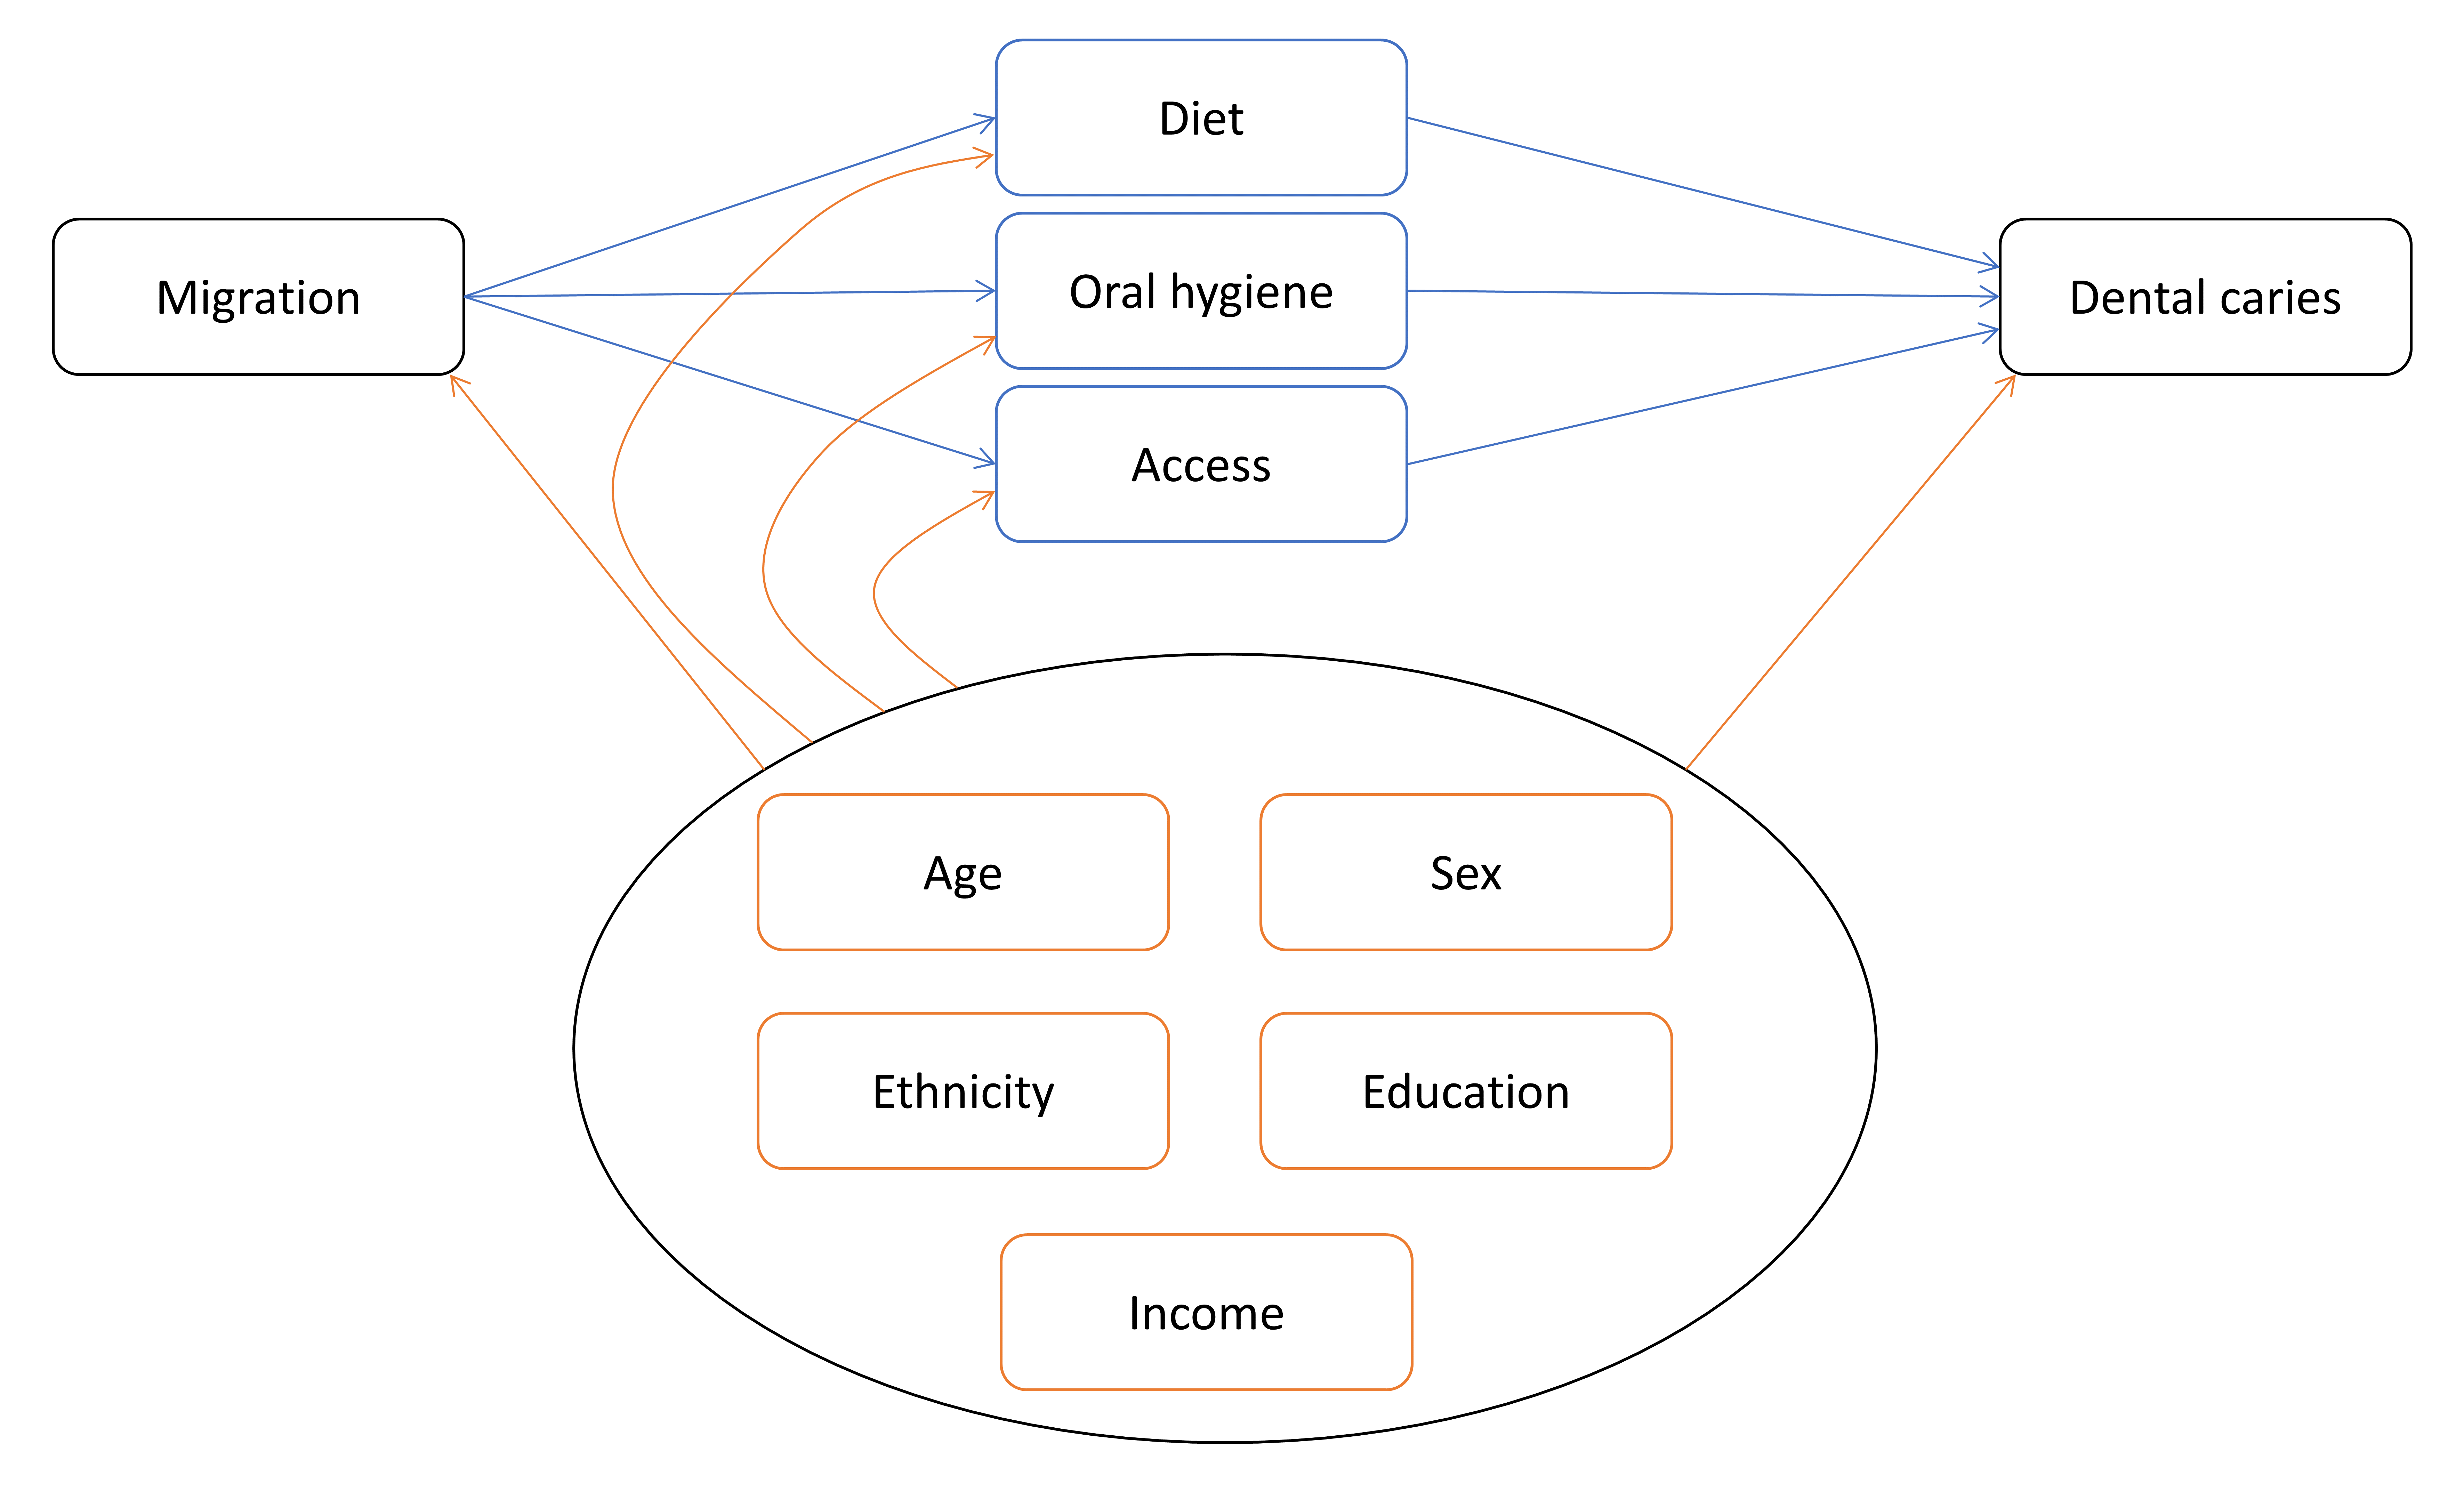
\includegraphics[scale = 0.5]{images/dag}
\caption{Directed acyclic graph showing mediating (blue) and confounding (orange) pathways linking migration and dental caries.}
\label{fig:dag}
\end{figure}